\section{Discussão dos Resultados}

Observamos que os modelos \textit{XGBoost} e \textit{LighGBM} tiveram os melhores desempenhos em validação e teste. O \textit{LighGBM} apresenta a vantagem de ser muito mais rápido em treinamento se comparado aos demais modelos, fato esse que é somado com seu maior valor de KS para validação. Contudo, em teste, o \textit{XGBoost} apresentou o melhor resultado (KS de 27.1), sendo a escolha final do modelo.

\begin{figure}[h]
\centering
\caption{\label{figure:figura3}Curvas ROC dos modelos \textit{XGBoost} e \textit{LighGBM}}
  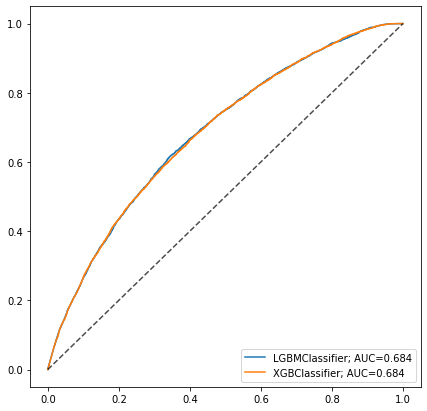
\includegraphics[width=0.4\textwidth,height=70mm]{assets/auc_roc.png}
  \\ Fonte: Condução dos experimentos pelos autores do artigo.
\end{figure}

Plotamos as curvas ROC e o valor de AUC para ambos modelos mencionados, de maneira a entender suas diferenças, apesar da diferença nos valores de KS em teste; as curvas são bem próximas, e possuem o mesmo valor de AUC. De maneira a entender se existem diferenças significativas entre os modelos supracitados, utilizamos o teste \textit{Wilcoxon} (pareado e não paramétrico), conduzindo 10 vezes os experimentos (\textit{k-fold}) com os algoritmos. Ao fim, o teste resultou em um p-valor dacima do limiar estabelecido (5\%), indicando que não existem diferenças significativas entre os modelos treinados.